\documentclass{article}

\usepackage[margin=1in]{geometry}
\usepackage{indentfirst}
\usepackage{amsmath}

\usepackage{graphicx}
\usepackage{subcaption}

\title{Prediction of Annual Medical Cost}
\author{Bixuan LIU}
\date{\today}


\begin{document}

\maketitle
	
\begin{abstract}

This project considers a dataset from kaggle, which has some information of clients from a health insurance company and their annual medical costs. It is very important for a health insurance company to predict the annual medical cost of a potential client, based on which the company can determine a reasonable premium. Therefore, in this project I implement four supervised machine learning methods, namely Gaussian Linear Model, Lasso, Regression Tree and Random Forest, to predict the annual medical costs, and select the best model for the task. Moreover, based on the results of this project, I'm able to design a short questionnaire for the potential clients of the health insurance company which will help them to predict the future annual medical costs and determine premiums.

\end{abstract}

\textbf{Keywords: } Health Insurance, Lasso, Random Forest

\newpage
\tableofcontents
\newpage

\section{Motivation}

It's very important for a health insurance company to make correct predictions of a potential client's annual medical cost, which is the foundation of determining a premium. Therefore, there are three main objectives for this project:
\begin{enumerate}
	\item Select the most appropriate machine learning method to predict the annual costs covered by health insurance of clients.
	\item Select the most influential factor(s) for the prediction of annual medical cost.
	\item Design a short questionnaire for the potential clients of the health insurance company.
\end{enumerate}

\section{Dataset}

\subsection{Source}
This dataset is from kaggle:
 https://www.kaggle.com/datasets/mirichoi0218/insurance?resource=download.
 
\subsection{Description}
The data is information collected from the clients of a health insurance company. It contains each client's individual medical costs billed by health insurance and several features of the client which may contribute to the costs. Names and descriptions of the entries are listed below:
\begin{itemize}
	\item \textbf{age}: age of primary beneficiary;
	\item \textbf{sex}: insurance contractor gender, female, male;
	\item \textbf{bmi}: body mass index;
	\item \textbf{children}: number of children covered by health insurance / number of dependents;
	\item \textbf{smoker}: smoking;
	\item \textbf{region}: the beneficiary's residential area in the US, northeast, southeast, southwest, northwest;
	\item \textbf{charges}: individual medical costs billed by health insurance.
\end{itemize}
See table \ref{tab:dataset} for the first three rows of the dataset as an example.
\begin{table}[h]
	\centering
	\begin{tabular}{|c|c|c|c|c|c|c|}
		\hline
		age & sex & bmi & children & smoker & region & charges \\
		\hline
		19 & female & 27.9 & 0 & yes & southwest & 16884.924 \\
		\hline
		18 & male & 33.77 & 1 & no & southeast & 1725.5523\\
		\hline
		28 & male & 33 & 3 & no & southeast & 4449.462 \\
		\hline
	\end{tabular}
	\caption{First Three Rows of Dataset}
	\label{tab:dataset}
\end{table}

\subsection{Visualization}
From table \ref{tab:dataset}, it's clear that the dataset contains both numerical (age, bmi, and charges) and categorical (sex, children, smoker, and region) entries. Next, I visualize these entries separately.
\begin{figure}[!ht]
	\centering
	
	\begin{subfigure}{0.45\textwidth}
		\centering
		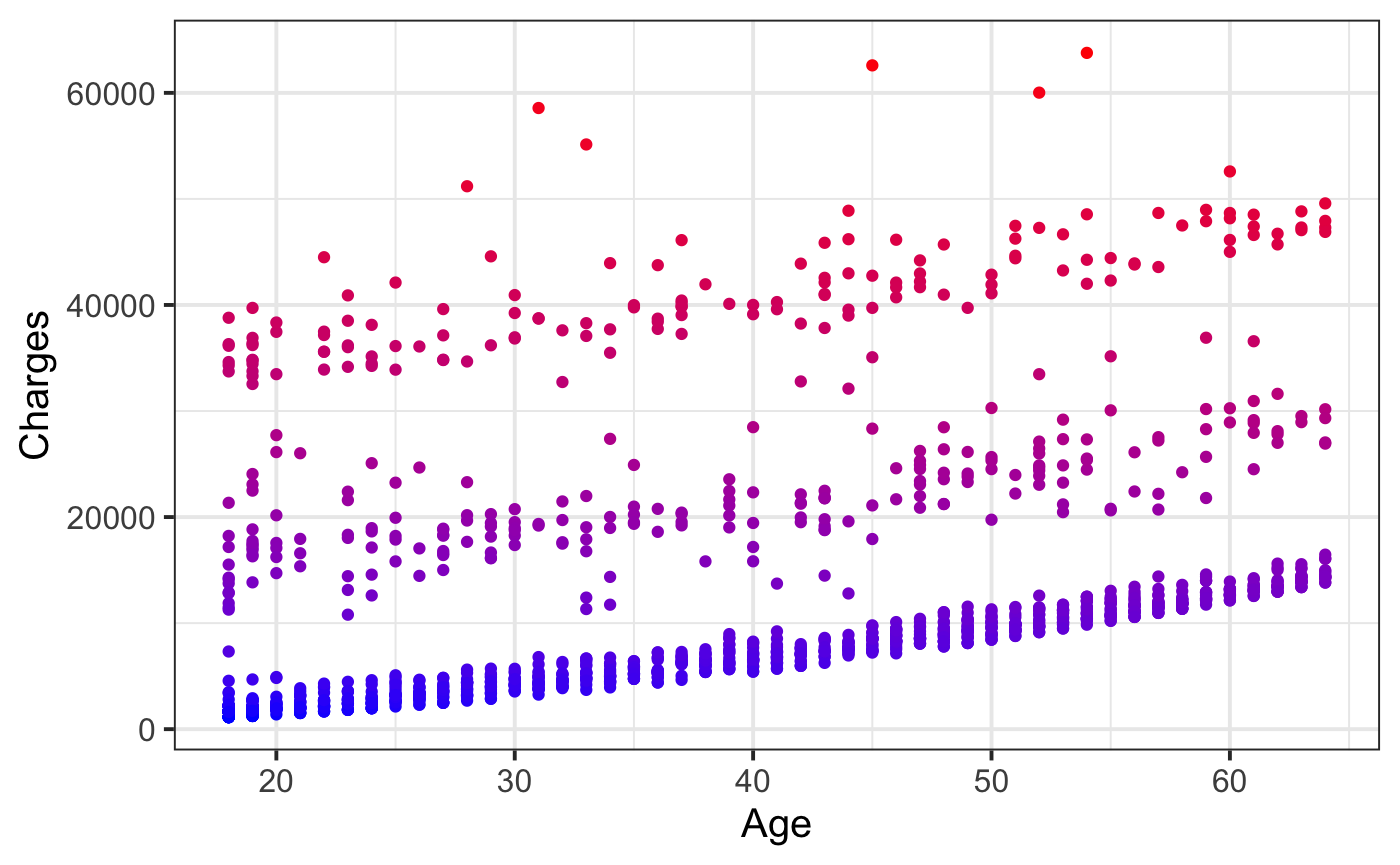
\includegraphics[width=\linewidth]{images/age_charges.png}
		\label{fig:age_charges}
	\end{subfigure}
	\hspace{0.05\textwidth} % Adjust the horizontal space between subfigures
	\begin{subfigure}{0.45\textwidth}
		\centering
		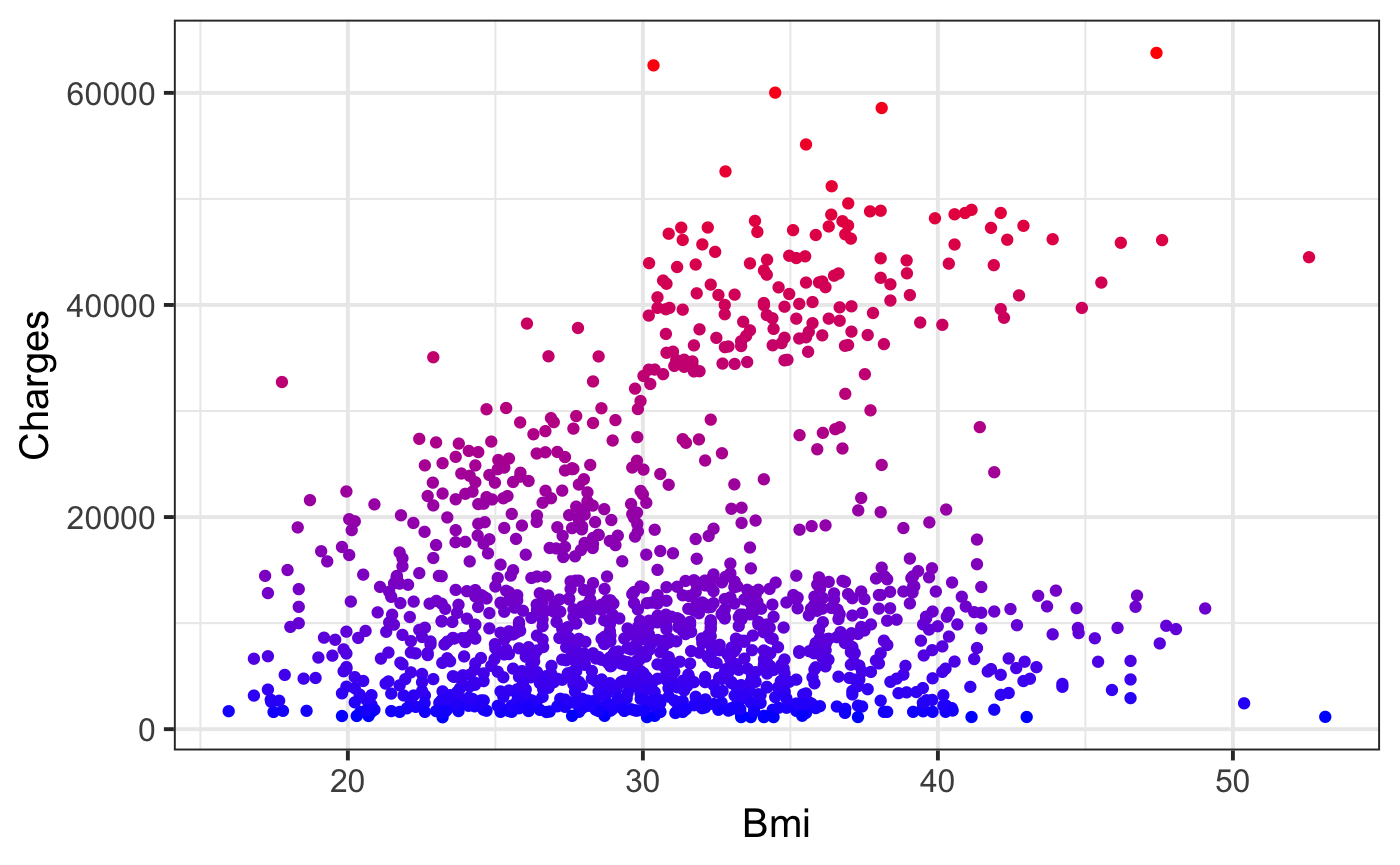
\includegraphics[width=\linewidth]{images/bmi_charges.png}
		\label{fig:bmi_charges}
	\end{subfigure}

	\caption{Age and Bmi vs Charges}
	\label{fig:age_bmi_charges}
\end{figure}

\begin{figure}[!ht]
	\centering
	
	\begin{subfigure}{0.45\textwidth}
		\centering
		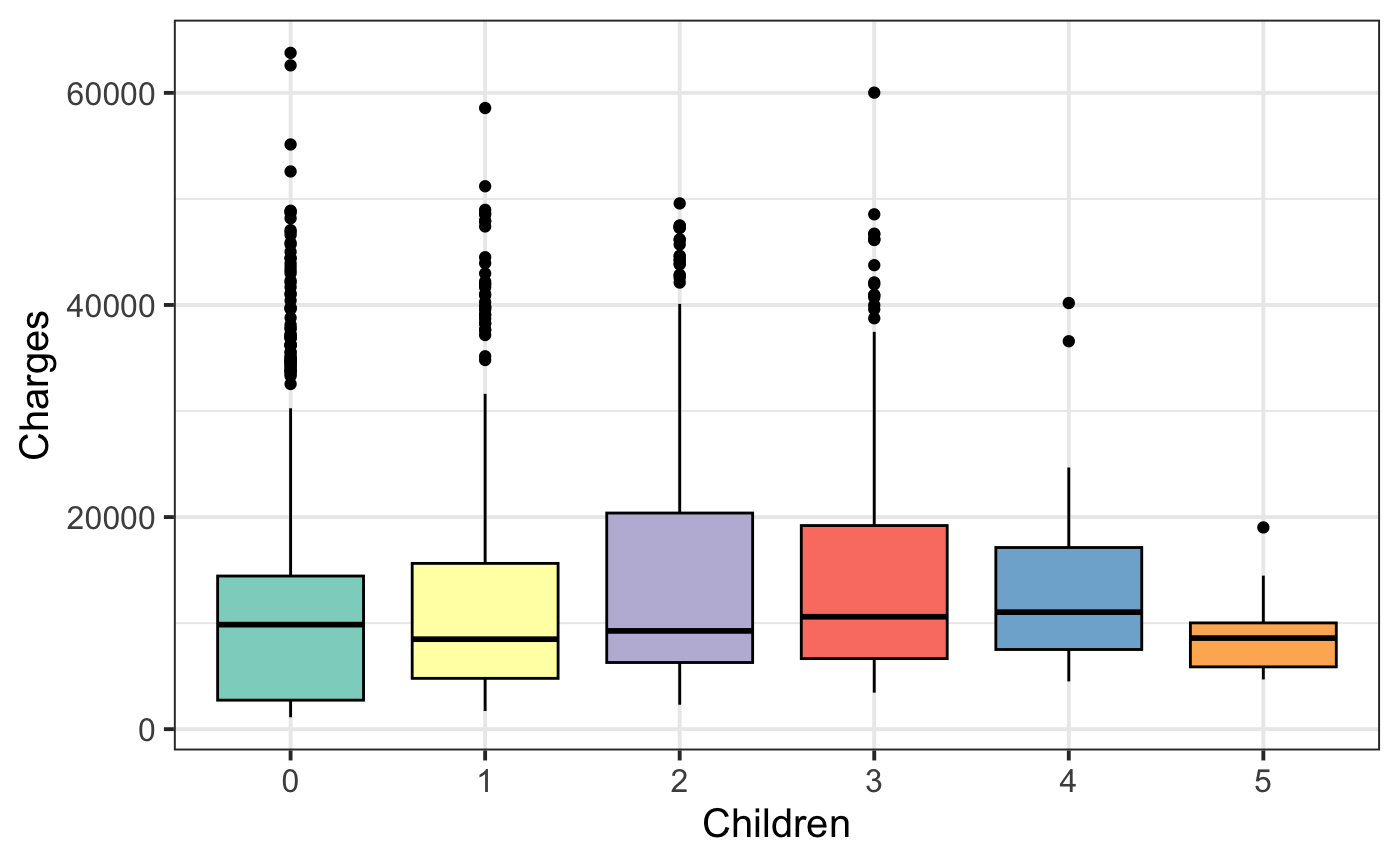
\includegraphics[width=\linewidth]{images/children_charges.png}
		\label{fig:children_charges}
	\end{subfigure}
	\hspace{0.05\textwidth} % Adjust the horizontal space between subfigures
	\begin{subfigure}{0.45\textwidth}
		\centering
		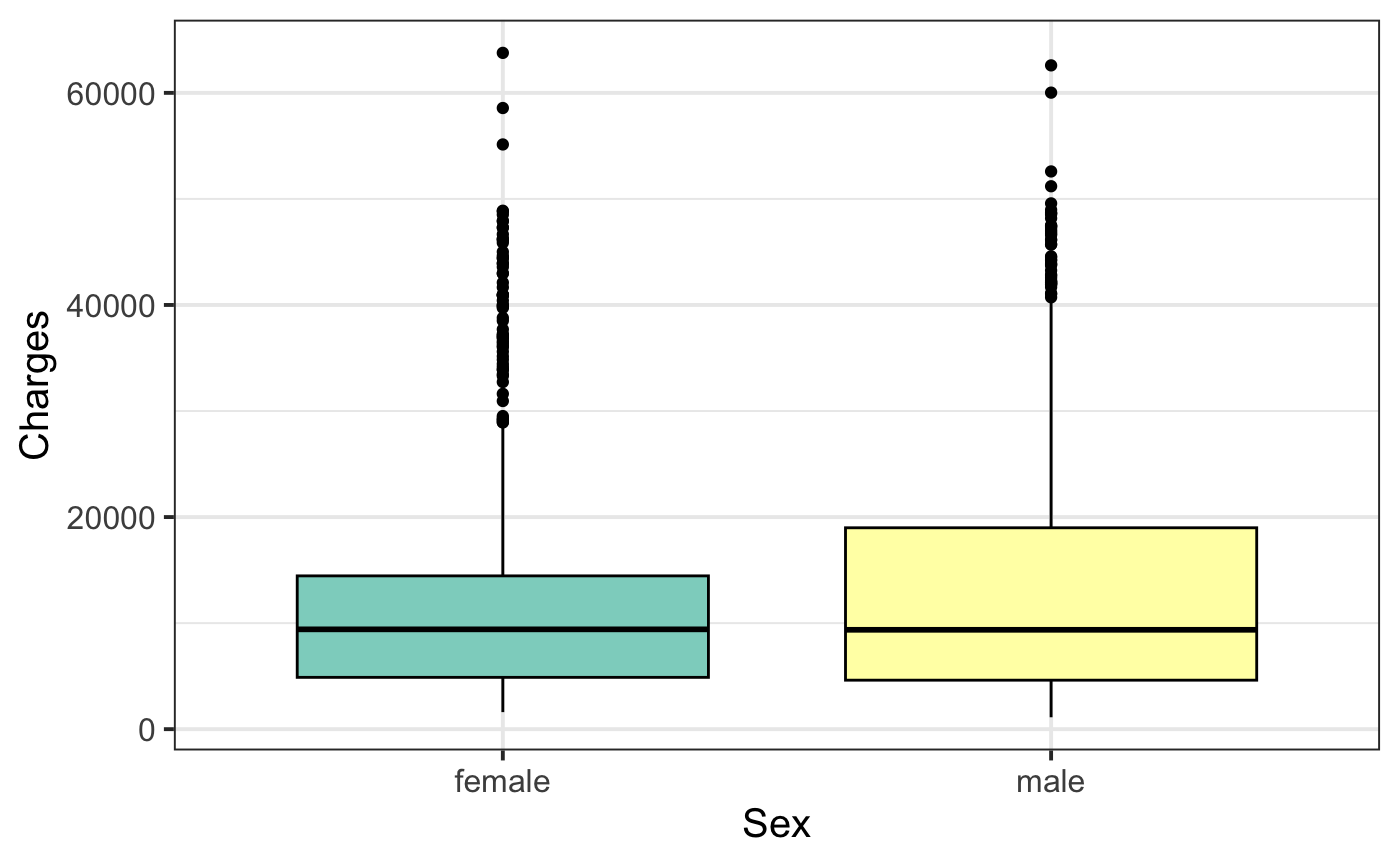
\includegraphics[width=\linewidth]{images/sex_charges.png}
		\label{fig:sex_charges}
	\end{subfigure}
	
	\vspace{0.5cm} % Adjust the vertical space between rows
	
	\begin{subfigure}{0.45\textwidth}
		\centering
		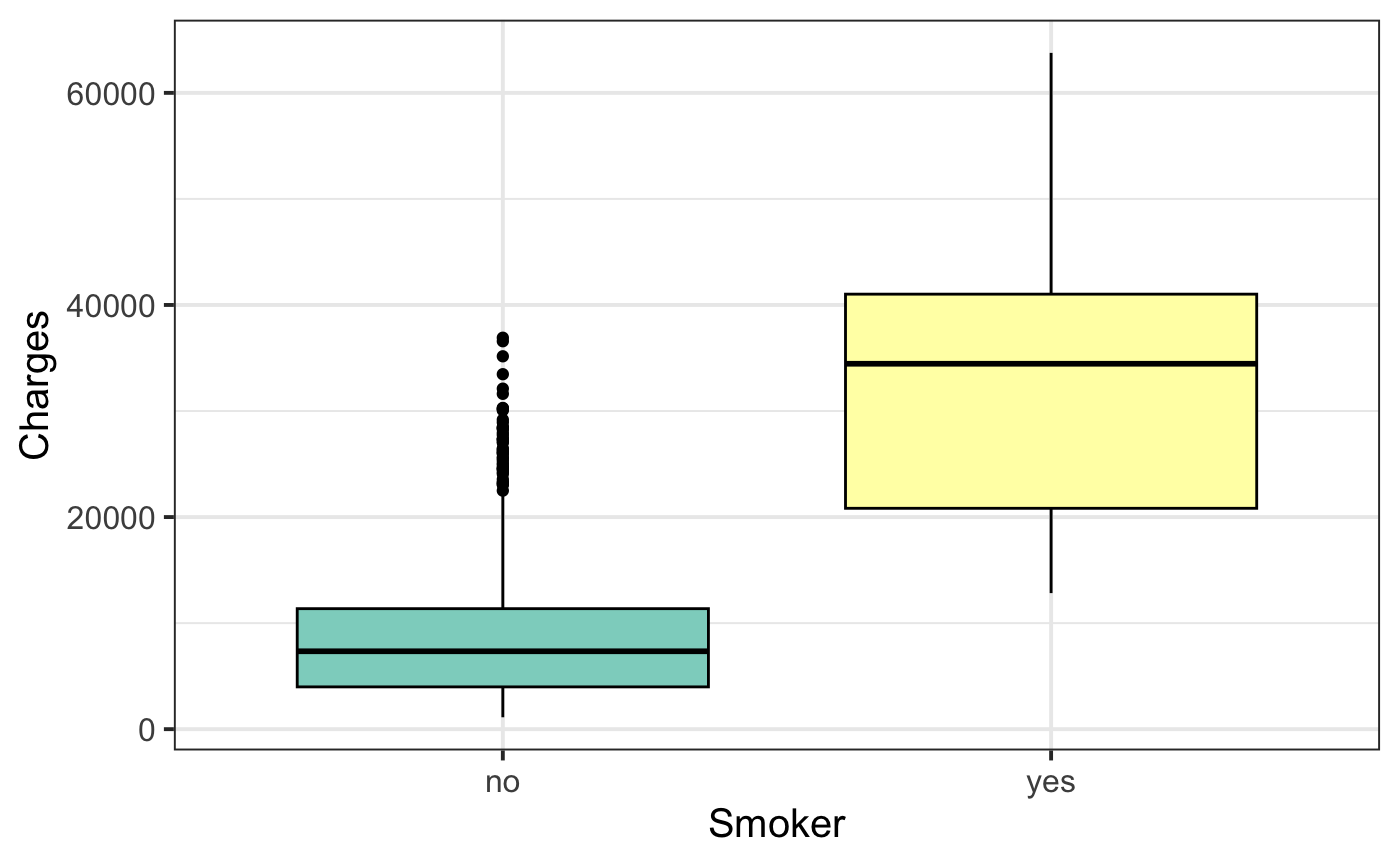
\includegraphics[width=\linewidth]{images/smoker_charges.png}
		\label{fig:smoker_charges}
	\end{subfigure}
	\hspace{0.05\textwidth} % Adjust the horizontal space between subfigures
	\begin{subfigure}{0.45\textwidth}
		\centering
		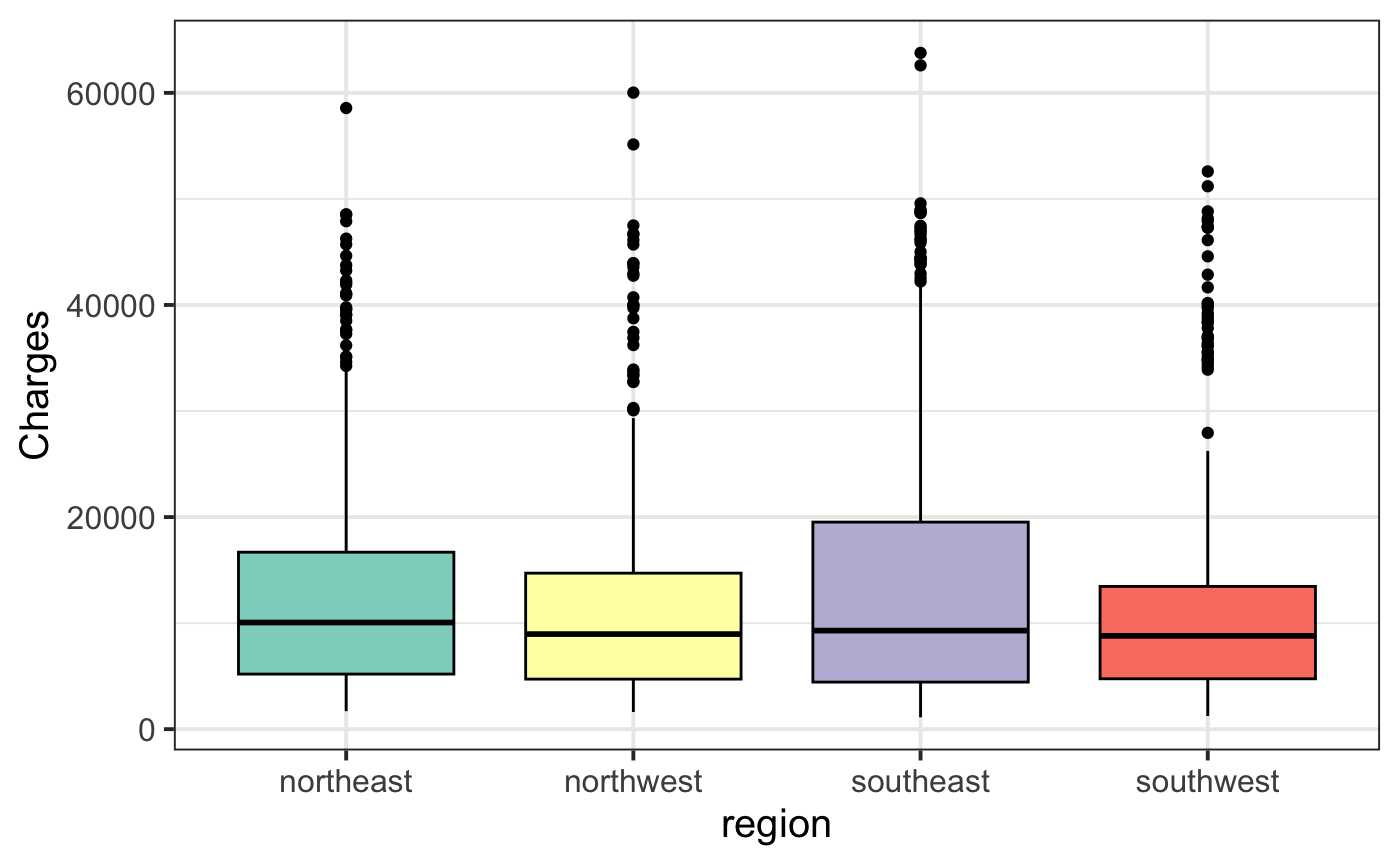
\includegraphics[width=\linewidth]{images/region_charges.png}
		\label{fig:region_charges}
	\end{subfigure}
	
	\caption{Children, Sex, Smoker and Region vs Charges}
	\label{fig:children_sex_smoker_region_charges}
\end{figure}
From figures \ref{fig:age_bmi_charges} and \ref{fig:children_sex_smoker_region_charges}, we can already observe some patterns about annual medical charges. There are three important columns: age, bmi and smoker, while the others do not show significant relations with the charges.

\section{Model Selection}

In this section, I consider the following four machine learning methods:
\begin{itemize}
	\item Gaussion Linear Model;
	\item Lasso;
	\item Regression Tree;
	\item Random Forest.
\end{itemize}
The purpose of this section is to select the best model for the prediction of annual charges and selection of important variable(s) that contribute(s) the most to the prediction.

\subsection{Steps for Fitting each Model to the Data}
\begin{itemize}
	\renewcommand{\labelitemi}{--}
	\item \textbf{Step 1,} split the dataset into $80\%$ of training and $20\%$ of testing set randomly.
	\item \textbf{Step 2,} fit the model to training set.
	\item \textbf{Step 3,} calculate the studendized residuals of training set, detect outliers and remove them.
	\item \textbf{Step 4,} fit again the model to cleaned training set and evaluate the model.
	\item \textbf{Step 5,} calculate RMSFE (Root Mean Squared Forecast Error) on the test set.
\end{itemize}

\subsection{Gaussian Linear Model}
Gaussian Linear Model is generally represented as:
\begin{equation}
	\label{eq:glm}
	Y = X\theta + \epsilon
\end{equation}
where $Y$ is of dimension $n \times 1$, representing the response variable (variable to be predicted) of $n$ observations. $Y_i$'s are assumed to be independent and Gaussian distributed. $X$ is of dimension $n \times \left(p + 1\right)$, representing $n$ observations of $p$ explanatory variables and $1$ constant.  $\theta$ is of dimension $\left(p + 1\right) \times 1$, representing fixed and unknown parameters. $\epsilon$ is of dimension $n \times 1$, representing the residuals. Here, we assume $\epsilon$'s are independently, identically distributed as $\mathcal{N} \sim \left(0,\sigma^2\right)$.

When applying Gaussian Linear Model to the dataset, categorical columns are transfered into numerical using one-hot-encoding. After fitting the model directly to training data, we get $R^2$ equals $74.32\%$, which is fairly good. Next, I use studentized residuals to detect outliers (see figure \ref{fig:outlier_glm}). 57 outliers are detected.
\begin{figure}[!ht]
	\centering
	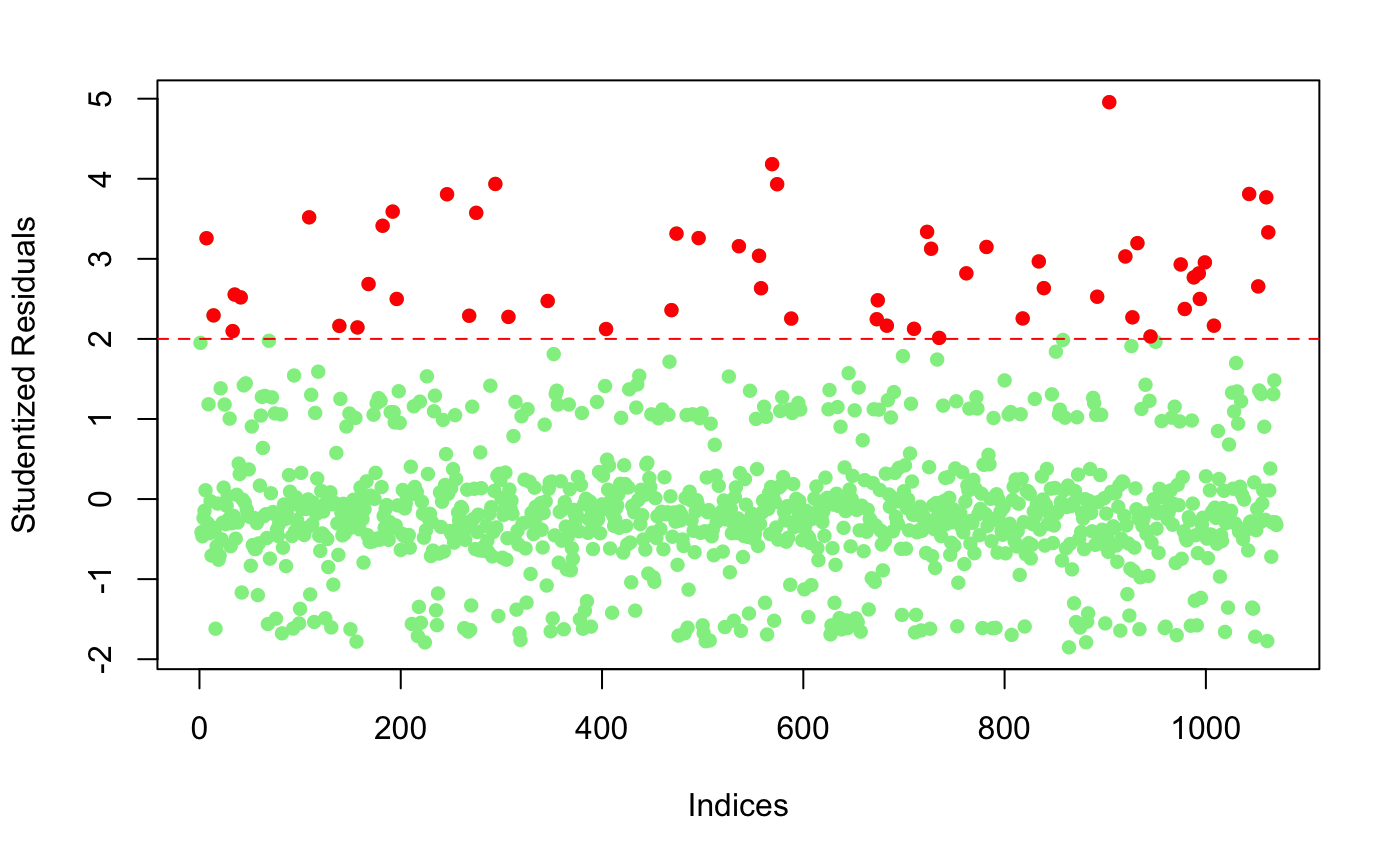
\includegraphics[width=0.8\linewidth]{images/outlier_glm.png}
	\caption{Outlier Detection for Gaussian Linear Model}
	\label{fig:outlier_glm}
\end{figure}

After removing the outliers in the training set, I fit again the model to the cleaned training set. The new $R^2$ value is $84.13\%$, which is improved compared to the previous model. The coefficients are listed in table \ref{tab:coef_glm}. 
\begin{table}[h]
	\centering
	\begin{tabular}{|l|r|}
		\hline
		Attribute & Estimated Coefficient \\
		\hline
		Intercept & -12931.42 \\
		\hline
		age & 256.63 \\
		\hline
		sexfemale & -235.26 \\
		\hline
		bmi & 338.98 \\
		\hline
		children & 256.63 \\
		\hline
		smokeryes & 256.63 \\
		\hline
		regionsoutheast & -940.62 \\
		\hline
		regionnorthwest & -341.06 \\
		\hline
		regionsouthwest & -429.29 \\
		\hline
	\end{tabular}
	\caption{Coefficients Estimated by Gaussian Linear Model}
	\label{tab:coef_glm}
\end{table}
See figure \ref{fig:dis_res_glm} for the distribution of standardized residuals.
\begin{figure}[!ht]
	\centering
	
	\begin{subfigure}{0.45\textwidth}
		\centering
		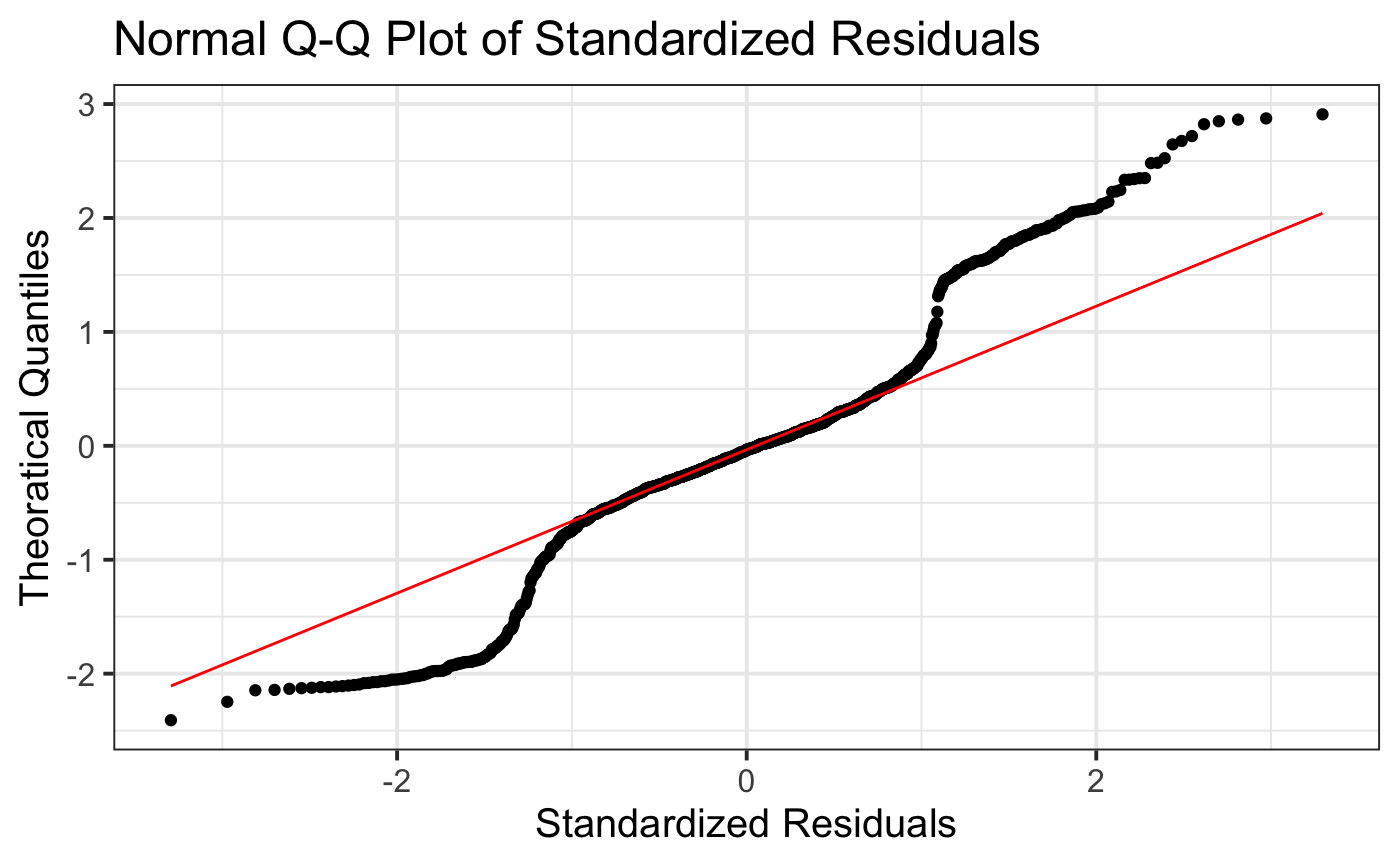
\includegraphics[width=\linewidth]{images/qq_glm.png}
		\label{fig:qq_glm}
	\end{subfigure}
	\hspace{0.05\textwidth} % Adjust the horizontal space between subfigures
	\begin{subfigure}{0.45\textwidth}
		\centering
		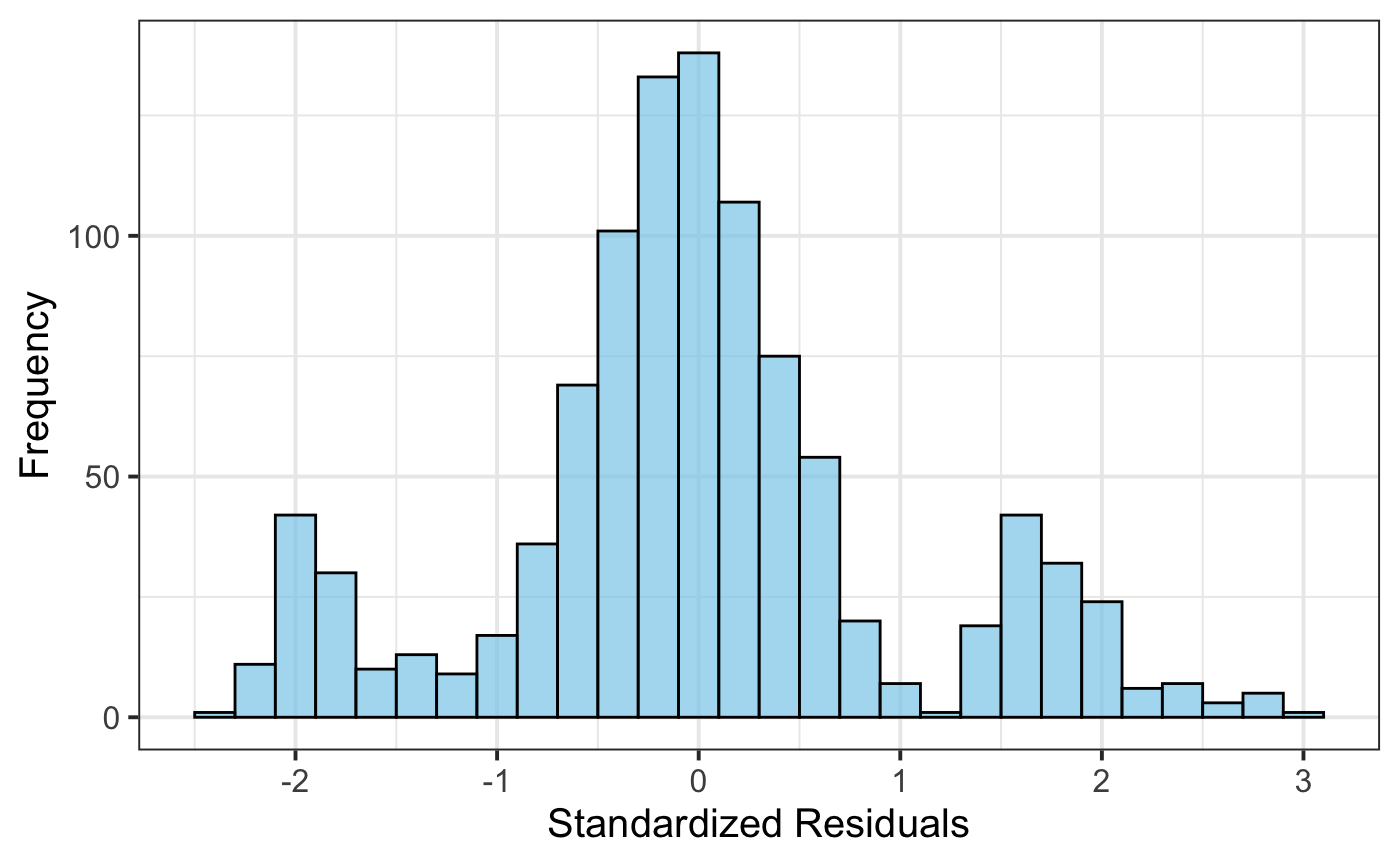
\includegraphics[width=\linewidth]{images/his_glm.png}
		\label{fig:his_glm}
	\end{subfigure}
	
	\caption{Distribution of Standardized Residuals of Gaussian Linear Model}
	\label{fig:dis_res_glm}
\end{figure}
The distribution of standardized residuals is fairly close to a normal distribution, which means that Gaussian Linear Model generally captures the relations between the variables. But clearly linear models are not the best choice since there clearly are some nonlinear patterns in the data. 

\subsection{Lasso}
Lasso is one of the most influential penalized methods in machine learning. Lasso estimator is the solution of the following optimization problem:
\begin{equation}
	\label{eq:lasso}
	\hat{\beta}_L =  \arg \min_{\beta} \left\{\sum_{i = 1}^{n} \left(Y_i - \beta_0 - \sum_{j = 1}^{p} X_{i,j}\beta_j \right)^2 + \lambda \|\beta\|_1\right\}
\end{equation}
By penalizing the loss function with $l_1$-norm, Lasso plays an important rule not only in prediction, but also in variable selection.

Since Lasso is particularly sensitive to the scale of the features, first I scale the columns: age, bmi and children to $0\sim 1$, and then fit the model to training data. Since Lasso is another linear model, here I don't list the detailed results of coefficients and distributions of residuals anymore, and focus on variable selection instead.

When I set $\lambda$ in equation \ref{eq:lasso} big enough, $500$ for example (table \ref{tab:coef_lasso}), Lasso is able to select the following 4 variables: age, bmi, children, smokeryes, and set the coefficients of other features to $0$.
\begin{table}[!ht]
	\centering
	\begin{tabular}{|l|r|}
		\hline
		Attribute & Estimated Coefficient \\
		\hline
		Intercept & 8715.7824 \\
		\hline
		age & 3276.0246 \\
		\hline
		sexfemale & 0 \\
		\hline
		sexmale & 0 \\
		\hline
		bmi & 1489.3908 \\
		\hline
		children & 127.6906 \\
		\hline
		smokeryes & 22385.9093 \\
		\hline
		regionsoutheast & 0 \\
		\hline
		regionnorthwest & 0 \\
		\hline
		regionsouthwest & 0 \\
		\hline
	\end{tabular}
	\caption{Coefficients Estimated by Lasso with $\lambda = 500$}
	\label{tab:coef_lasso}
\end{table}
It's also worth mentioning that from the absolute values of the coefficients, we can conclude that in the four selected features, smoker is the most influential while children is the least.

\subsection{Regression Tree and Random Forest}
Unlike above mentioned methods, regression tree builds a decision tree with certain nodes and leaves that can capture non-linear relationships. In this section, I only show the results with cleaned training set, the process of detecting outliers are omitted.

Figure \ref{fig:tree_structure} gives an instance of the first two layers of the regression tree built on the cleaned training set. The model has $R^2$ equals $93.42\%$, which is fairly high, suggesting that the model fits very well with the training data. 
\begin{figure}[!ht]
	\centering
	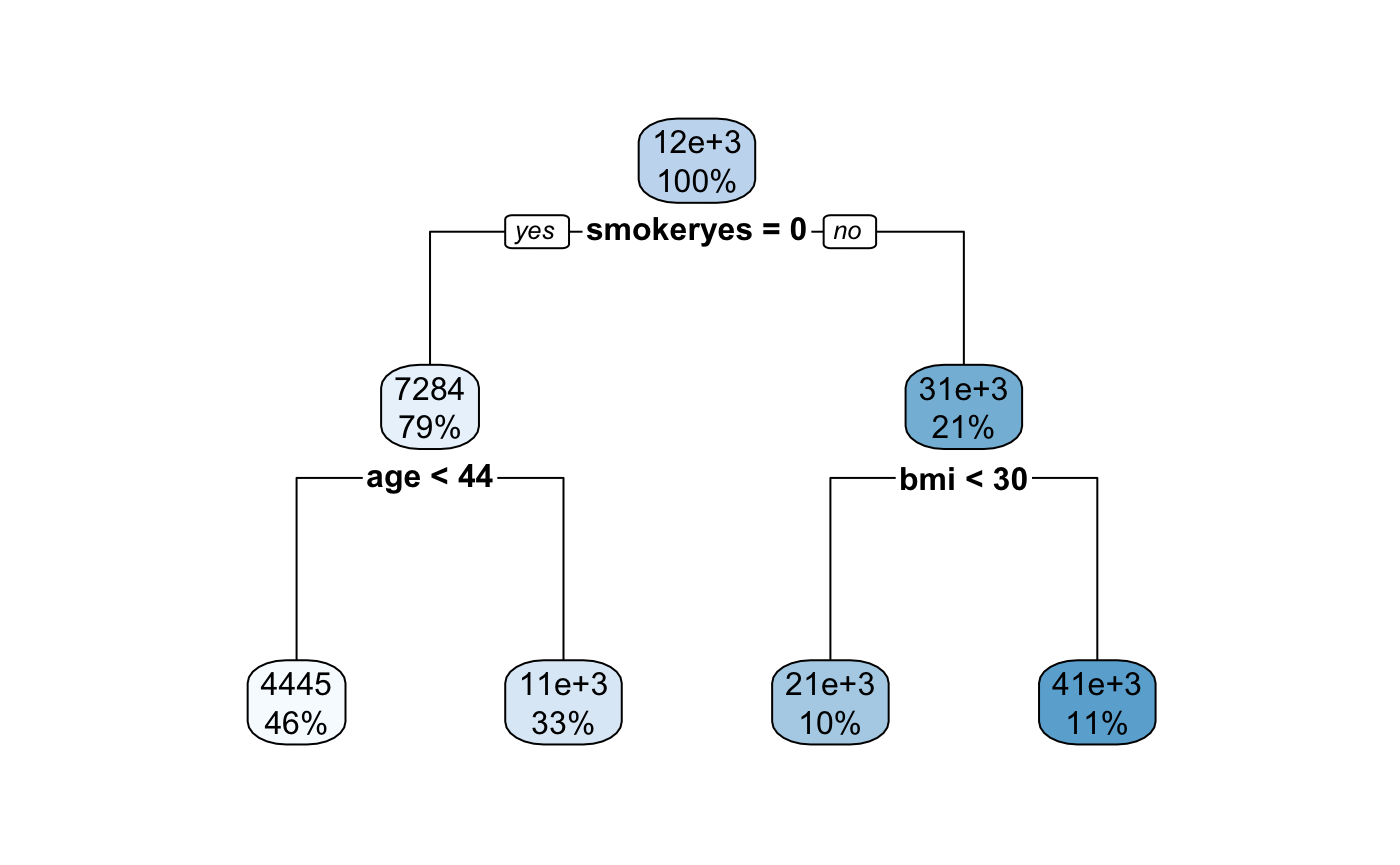
\includegraphics[width=0.8\linewidth]{images/tree_structure.png}
	\caption{Instance of Regression Tree Structure}
	\label{fig:tree_structure}
\end{figure}

Random forest is a combination of several regression trees, which should behave better than simple regression tree. After fitting a random forest with $100$ regression trees to the training set, $R^2$ becomes $95.70\%$. Figure \ref{fig:dis_res_forest} shows the behavior of the residuals.
\begin{figure}[!ht]
	\centering
	
	\begin{subfigure}{0.45\textwidth}
		\centering
		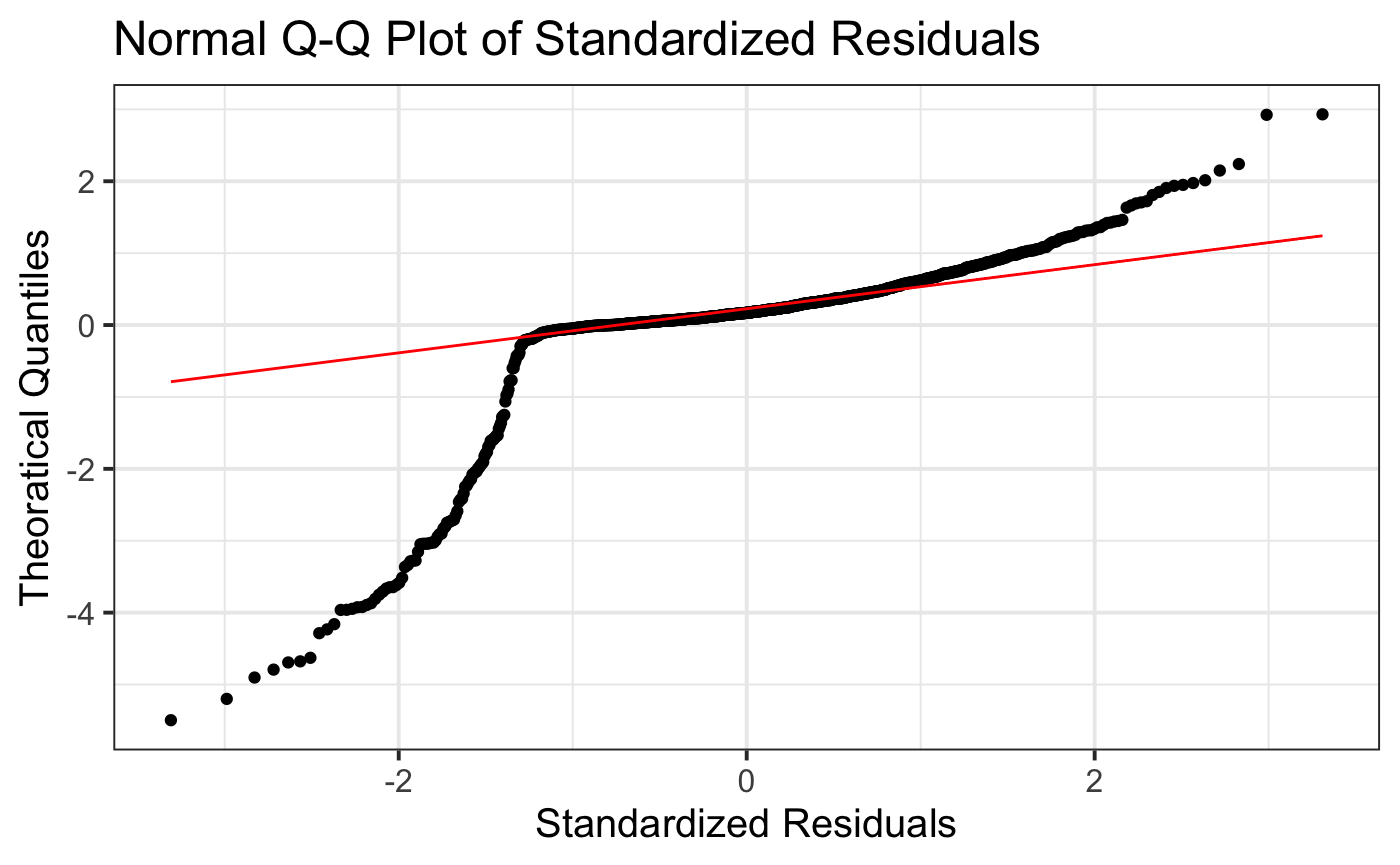
\includegraphics[width=\linewidth]{images/qq_forest.png}
		\label{fig:qq_forest}
	\end{subfigure}
	\hspace{0.05\textwidth} % Adjust the horizontal space between subfigures
	\begin{subfigure}{0.45\textwidth}
		\centering
		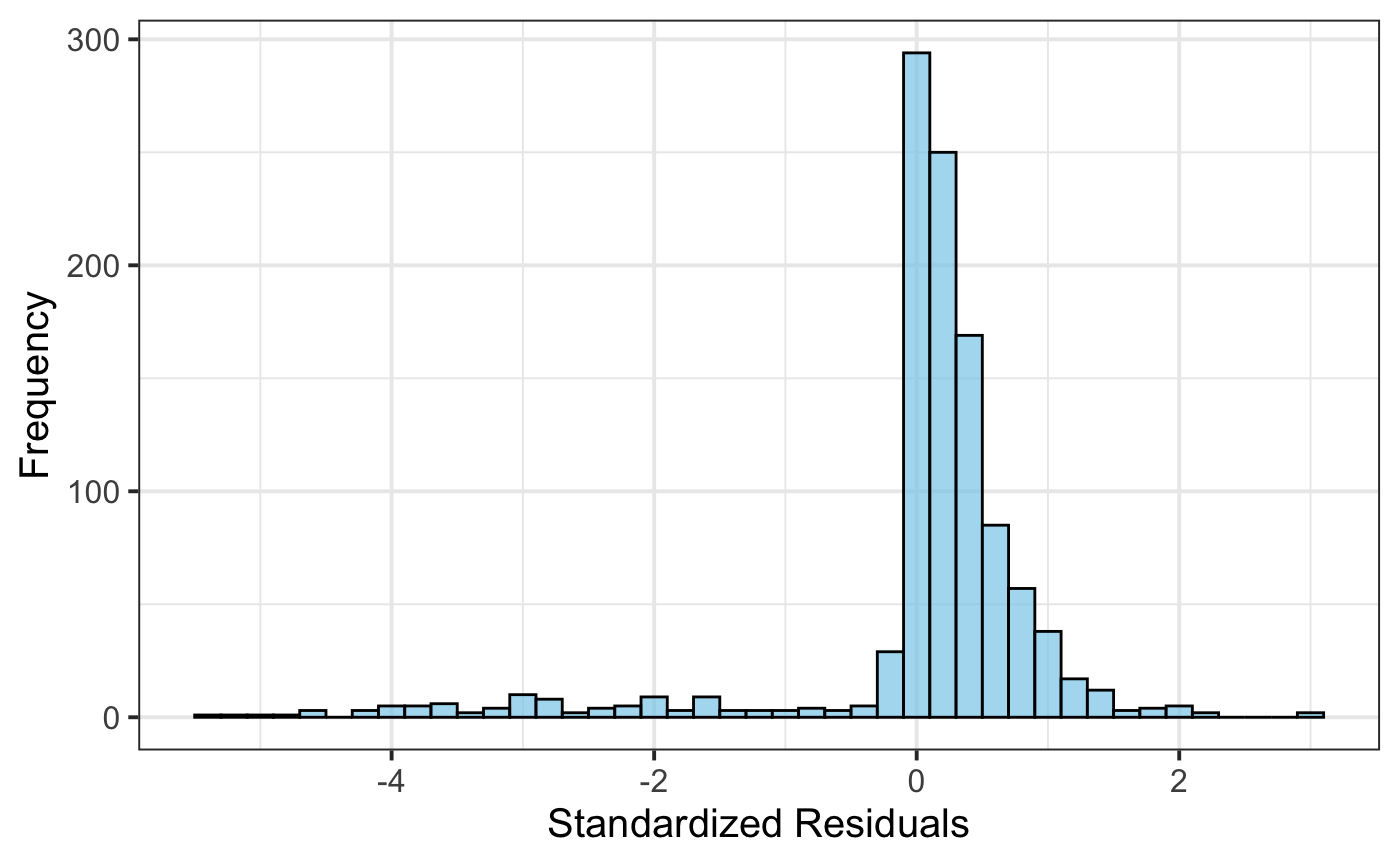
\includegraphics[width=\linewidth]{images/his_forest.png}
		\label{fig:his_forest}
	\end{subfigure}
	
	\caption{Distribution of Standardized Residuals of Random Forest}
	\label{fig:dis_res_forest}
\end{figure}

\section{Conclusion}

Table \ref{tab:comp_mdl} shows the comparison of all models. It's clear that Random Forest is the best among the four methods considered in this project. And it reaches a lowest root mean squared forecast error of $0.32$.
\begin{table}[!ht]
	\centering
	\begin{tabular}{|c|c|c|c|c|}
		\hline
		Model & GLM & Lasso & Regression Tree & Random Forest \\
		\hline
		$R^2\left(\%\right)$ & 74.32 & 75.62 & 93.41 & 95.69 \\
		\hline
		$RMSFE$ & 0.43 & 0.43 & 0.37 & 0.32 \\
		\hline
	\end{tabular}
	\caption{Comparison of All Models}
	\label{tab:comp_mdl}
\end{table}

Based on all the results above, if I need to design a questionnaire for the insurance company, the three questions that should be asked are:
\begin{enumerate}
	\item How old are you?
	\item Do you smoke?
	\item What's your bmi?
\end{enumerate}
With the answers to the above questions, the insurance company will be able to make a fair prediction on the potential client's annual medical cost and define a premium.

\end{document}